\section{Diseño y arquitectura de la aplicación}
\label{sec:diseñoArquitectura}

\subsection{Dominio de \textit{VSCode4Teaching}}
\label{subsec:arqDominio}
El proyecto \textit{VSCode4Teaching} es una herramienta cuyo dominio es un contexto educativo, por que los elementos de la realidad que es preciso modelar en la aplicación informática son los habitualmente presentes en este marco, en el que intervienen usuarios en dos roles diferenciados ---profesores y estudiantes--- y que se organiza en cursos compuestos por ejercicios sobre los que se hacen propuestas de resolución.

\begin{figure}[ht]
    \centering
    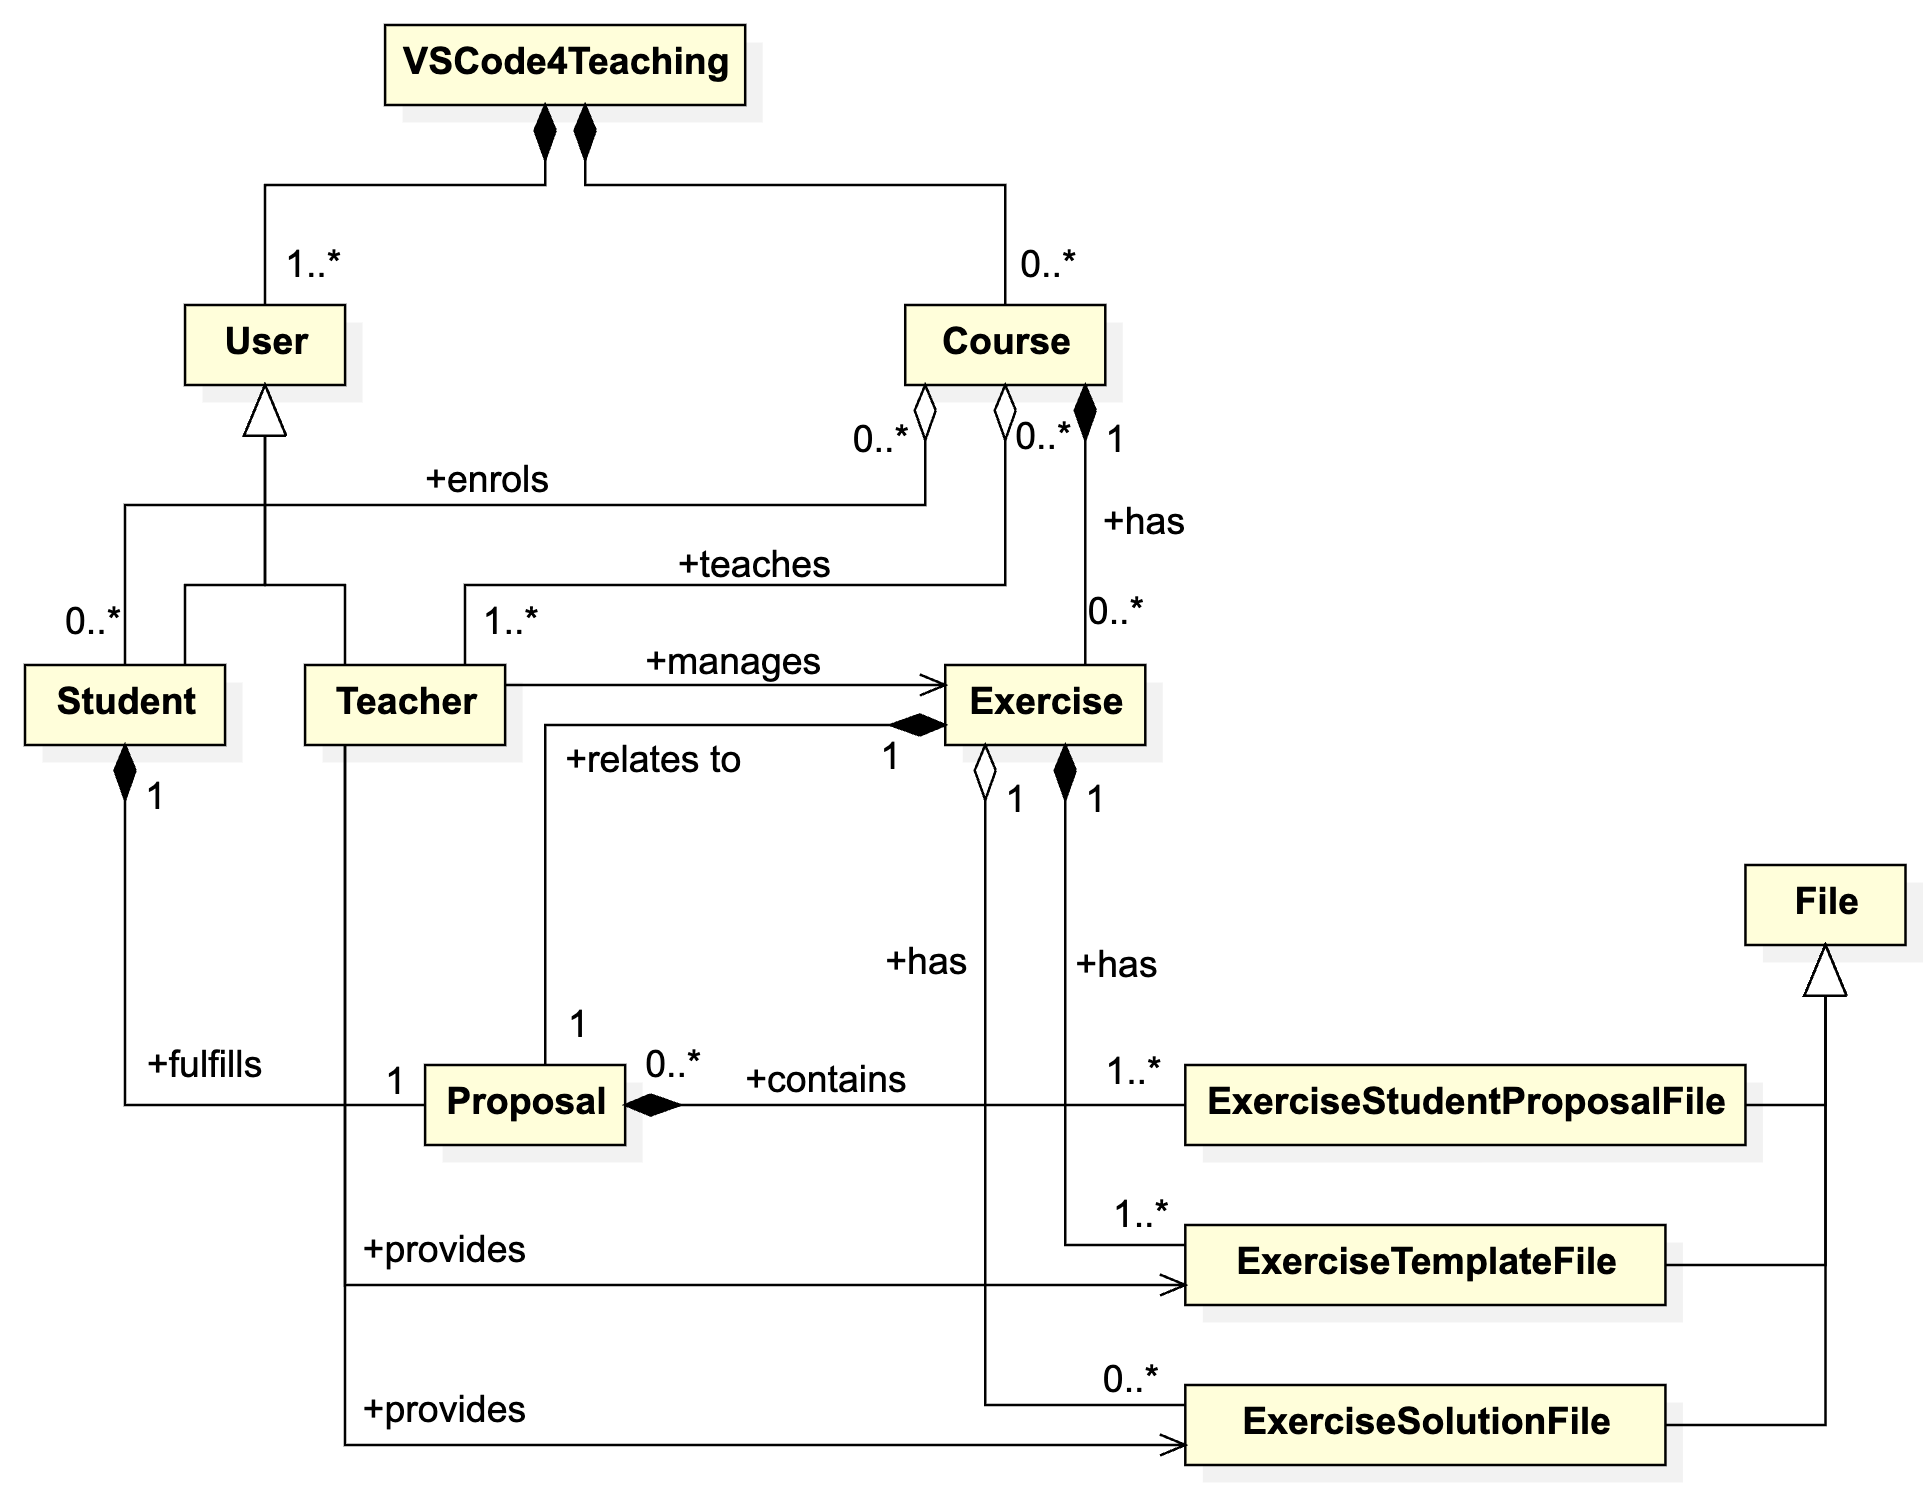
\includegraphics[width=\textwidth]{imagenes/utilizadas/4-2-arquitectura/diagramas/diag1-dominioAltoNivel.png}
    \caption{Representación en notación UML del dominio de \textit{VSCode4Teaching}.}
    \label{fig:diagDominioAltoNivel}
\end{figure}

La \referenciaFigura{fig:diagDominioAltoNivel} es un diagrama en notación UML\footnote{UML. Siglas de ``lenguaje unificado de modelado'' (del inglés \textit{Unified Model Language}). Es un convenio de diagramas de diversa índole para modelado estático y dinámico de \textit{software} muy extendido.} de los principales elementos del dominio de \textit{VSCode4Teaching} y sus interrelaciones en alto nivel, sirviendo como base para traducirlo a una agrupación de clases interrelacionadas que conformarán posteriormente el modelo que servirá de piedra angular de la herramienta informática implementada.

Esta definición esencial del dominio de la aplicación permite, por tanto, comprender mediante una notación estandarizada en el ámbito de la informática el conjunto de las entidades relevantes para la aplicación y cómo se relacionan y conectan entre sí. Este diagrama es el punto de partida sobre el que se construye el modelo empleado en los distintos componentes.

\subsection{Arquitectura del proyecto: organización de componentes}
\label{subsec:arq}
Previamente al inicio del presente TFG, \textit{VSCode4Teaching} disponía de dos componentes, tal como se muestra en la \referenciaFigura{fig:arquitecturaInicial}. En ella se aprecia una arquitectura cliente-servidor elemental en la que ambas partes se comunican haciendo uso de una API REST y de \textit{Web Sockets} \cite{IONOSWebSocket}, de modo que toda la lógica de la interpretación y persistencia de información en base de datos recae en el servidor; y su preparación para su visualización y la interacción con el usuario, en el cliente.

\begin{figure}[h]
    \centering
    \begin{tikzpicture}[
        > = latex',
        sistema/.style = {draw, minimum height=7mm,
                        inner sep=1mm, outer sep = 0mm}
        ]

        \node[sistema, fill={rgb,255: red,232; green,246; blue,229}] (servidor) {
            \begin{tabular}{cc}
                \multirow{2}{*}{
\includegraphics[height=0.7cm]{imagenes/utilizadas/4-2-arquitectura/logotipos/spring.png}} & Servidor \\
                                                                                               & \footnotesize{Spring Boot} \\
            \end{tabular}
        };
        \node[sistema, below=15mm of servidor, fill={rgb,255: red,250; green,239; blue,228}] (baseDatos) {
            \begin{tabular}{cc}
                \multirow{2}{*}{
\includegraphics[height=0.7cm]{imagenes/utilizadas/4-2-arquitectura/logotipos/mySQL.png}} & Base de datos \\
                                                                                              & \footnotesize{MySQL} \\
            \end{tabular}
        };
        \node[sistema, right=50mm of servidor, fill={rgb,255: red,215; green,243; blue,255}] (cliente) {
            \begin{tabular}{cc}
                \multirow{2}{*}{
\includegraphics[height=0.7cm]{imagenes/utilizadas/4-2-arquitectura/logotipos/vscode.png}} & Extensión\\
                                                                                               & \footnotesize{Visual Studio Code}\\
            \end{tabular}
        };

        \draw[<->] (servidor) -- node[above] {\scriptsize API REST + Web Sockets} (cliente);
        \draw[<->] (servidor) -- node[right] {\scriptsize Persistencia} (baseDatos);
    \end{tikzpicture}
    \caption{Fisonomía inicial de los componentes de la aplicación.}
    \label{fig:arquitecturaInicial}
\end{figure}

Esta fisonomía ha experimentado un proceso de ampliación durante la ejecución de esta tercera evolución del proyecto \textit{VSCode4Teaching}. Análogamente al diagrama anterior, en la \referenciaFigura{fig:arquitecturaFinal} se ilustra en alto nivel la arquitectura resultante tras la implementación de todos los requisitos.

Este diagrama refleja la modificacion arquitectónica más destacable realizada durante el Trabajo Fin de Grado: la introducción de la nueva aplicación web, que es el entorno sobre el que se ejecuta la implementación de algunos de los nuevos requisitos. Esta aplicación web se introduce como segundo cliente de la API publicada por el servidor, con el que se comunica mediante peticiones REST por HTTP\footnote{HTTP. Siglas de ``protocolo de transferencia de hipertexto'' (del inglés \textit{HyperText Transfer Protocol}).} del mismo modo en que lo hace la extensión de Visual Studio Code.

\begin{figure}[ht]
    \centering
    \begin{tikzpicture}[
        > = latex',
        sistema/.style = {draw, minimum height=7mm,
                        inner sep=1mm, outer sep = 0mm}
        ]

        \node[sistema, fill={rgb,255: red,232; green,246; blue,229}] (servidor) {
            \begin{tabular}{cc}
                \multirow{2}{*}{
\includegraphics[height=0.7cm]{imagenes/utilizadas/4-2-arquitectura/logotipos/spring.png}} & Servidor \\
                                                                                               & \footnotesize{Spring Boot} \\
            \end{tabular}
        };
        \node[sistema, above=10mm of servidor, fill={rgb,255: red,250; green,239; blue,228}] (baseDatos) {
            \begin{tabular}{cc}
                \multirow{2}{*}{
\includegraphics[height=0.7cm]{imagenes/utilizadas/4-2-arquitectura/logotipos/mySQL.png}} & Base de datos \\
                                                                                              & \footnotesize{MySQL} \\
            \end{tabular}
        };
        \node[sistema, below right=3mm and 1mm of servidor, fill={rgb,255: red,255; green,205; blue,216}] (appweb) {
            \begin{tabular}{cc}
                \multirow{2}{*}{
\includegraphics[height=0.7cm]{imagenes/utilizadas/4-2-arquitectura/logotipos/angular.png}} & Aplicación web\\
                                                                                               & \footnotesize{Angular}\\
            \end{tabular}
        };
        \node[sistema, below left=3mm and 1mm of servidor, fill={rgb,255: red,215; green,243; blue,255}] (cliente) {
            \begin{tabular}{cc}
                \multirow{2}{*}{
\includegraphics[height=0.7cm]{imagenes/utilizadas/4-2-arquitectura/logotipos/vscode.png}} & Extensión\\
                                                                                               & \footnotesize{Visual Studio Code}\\
            \end{tabular}
        };

        \draw[<->] (servidor.west) -| node[above] {\scriptsize API REST + Web Sockets} (cliente);
        \draw[<->] (servidor.east) -| node[above] {\scriptsize API REST} (appweb);
        \draw[<->] (servidor) -- node[right] {\scriptsize Persistencia} (baseDatos);
    \end{tikzpicture}
    \caption{Arquitectura final de alto nivel de los componentes de la aplicación.}
    \label{fig:arquitecturaFinal}
\end{figure}

\subsection{Diseño interno de cada componente}
\label{subsec:diseño}
Cada uno de los componentes introducidos en la \referenciaSeccion{subsec:arq} está conformado por un conjunto de clases e interfaces que quedan organizadas según patrones organizacionales o arquitectónicos adaptados para adecuarse a las necesidades del lenguaje o plataforma subyacente tras cada componente, pues la heterogeneidad de las tecnologías empleadas para la implementación de cada uno de ellos conlleva la adaptación de la organización a la especificidad de cada caso.

No obstante, la fisonomía de las arquitecturas resultantes en cada componente es muy similar, ya que todas toman como base el patrón Modelo-Vista-Controlador \cite{Arq_MVCFowler} (MVC), que establece una categorización en tres capas o niveles: la vista, encargada del intercambio de información con el usuario o el consumidor; el modelo, que refleja en clases interdependientes los objetos existentes en el dominio de la aplicación; y el controlador, que actúa como intermediario de las dos capas anteriores y contiene intrínsecamente la definición de los procesos de negocio implementados.

Esta similaridad entre los tres componentes hace posible realizar un modelo común a todos ellos, únicamente diferenciado en el lenguaje que los implementa en cada caso. Este modelo está basado en el dominio, introducido en la \referenciaSeccion{subsec:arqDominio}, sobre el que se interpretan las distintas entidades y sus conexiones para convertirlas en clases que contienen atributos de tipos primitivos, añadiendo así el detalle de la información relacionada con cada entidad; y que están interconectadas entre sí a través de atributos cuyos tipos son las propias clases generadas. Así, el dominio queda modelado en un conjunto de clases conectadas que forman la capa sustancial y fundamental de cada componente. El diagrama de clases UML incluido en la \referenciaFigura{fig:diagClasesModelo} es el reflejo de la capa de modelo implementada en el servidor, pero es prácticamente igual en los restantes componentes.

\begin{figure}[ht]
    \centering
    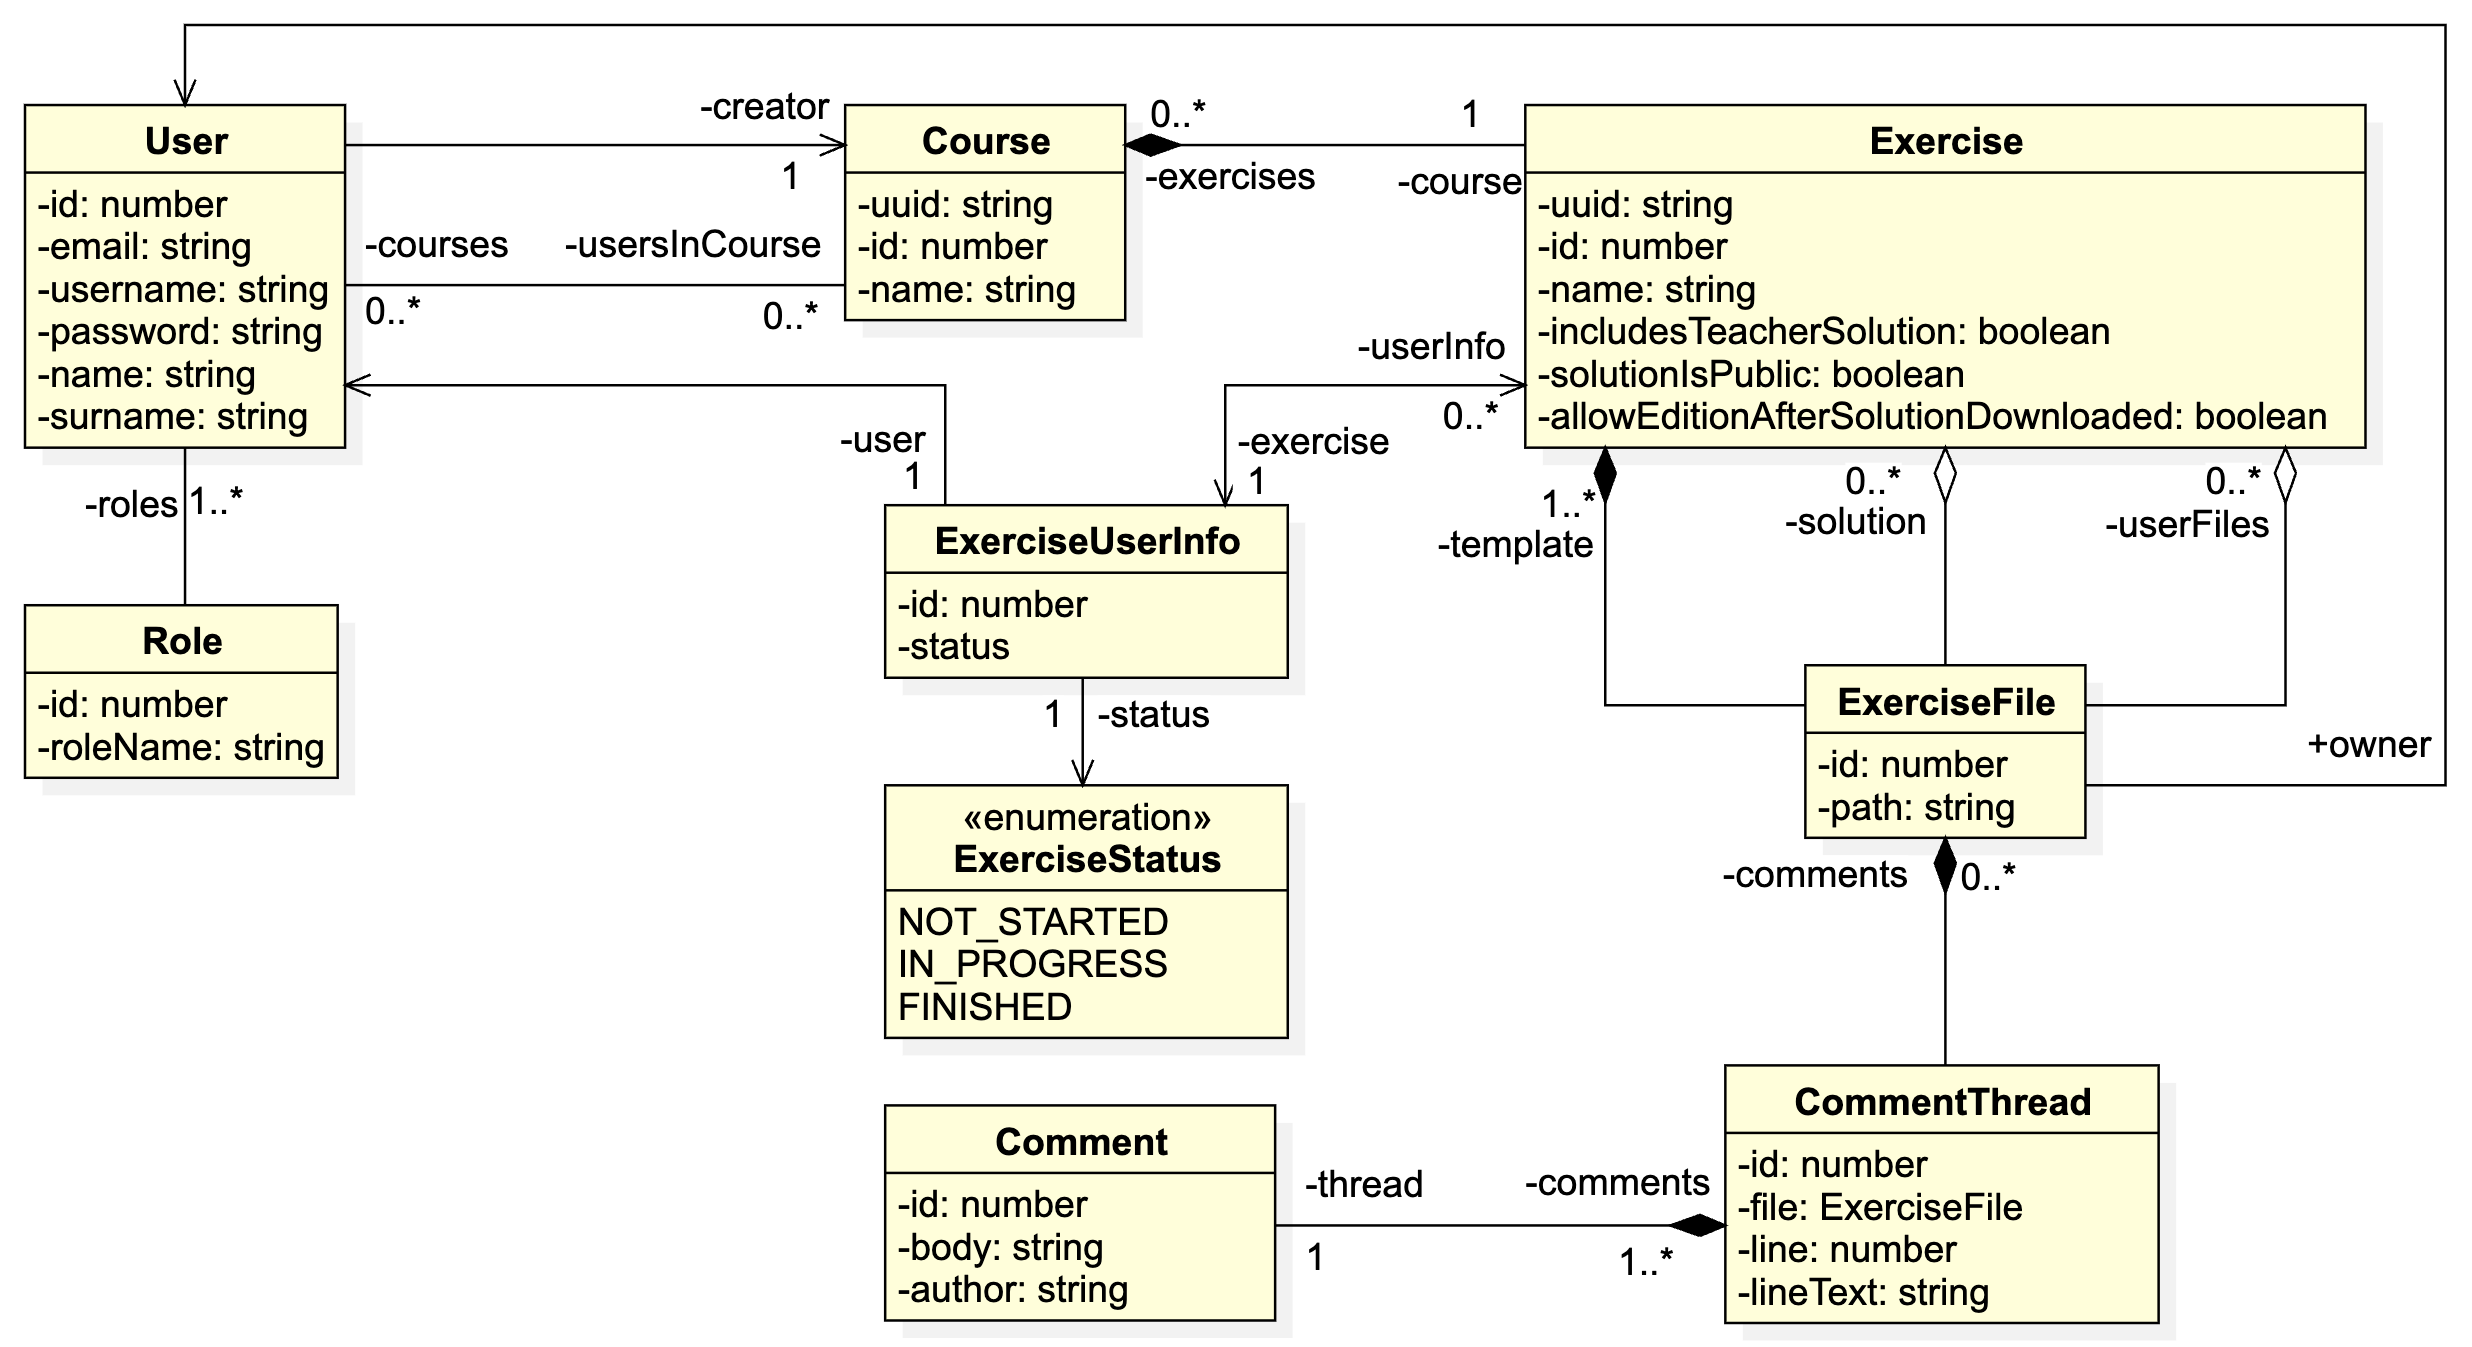
\includegraphics[width=\textwidth]{imagenes/utilizadas/4-2-arquitectura/diagramas/diag2-modeloDominioServidor.png}
    \caption{Diagrama de clases UML del modelo del dominio.}
    \label{fig:diagClasesModelo}
\end{figure}

Las siguientes subsecciones desarrollan la arquitectura de cada uno de los componentes: del servidor (\referenciaSeccion{subsec:arqServidor}), de la extensión (\referenciaSeccion{subsec:arqCliente}) y de la aplicación web (\referenciaSeccion{subsec:arqAppWeb}).

\subsubsection{Servidor}
\label{subsec:arqServidor}
El servidor es una aplicación Spring Boot ---véase la \referenciaSeccion{subsec:tecServidor}--- que sigue un patrón Modelo-Vista-Controlador (MVC) \cite{Arq_MVCFowler}. De este modo, el servidor se encuentra dividido en tres niveles asociados a cada una de las partes de la arquitectura MVC:
\begin{itemize}
    \item Modelo. Es la agrupación de todas las clases destinadas a la representación del dominio y sus interrelaciones. Al haber utilizado Spring Boot junto con Spring Data, además, estas clases sirven de referencia al ORM Hibernate para generar el esquema de base de datos y actúan como DTO\footnote{DTO. Siglas de ``objeto de transferencia de datos'' (del inglés \textit{Data Transfer Object}). Son instancias de clases cuyos atributos no toman su tipo del modelo específico de la aplicación y que se usan para transferir datos entre componentes o entre capas.} en la relación entre la base de datos y el servidor, que se realiza a través de interfaces repositorio que actúan como DAO\footnote{DAO. Siglas de ``objeto de acceso a datos'' (del inglés \textit{Data Access Object}). Son instancias de clases con métodos que permiten la interacción con sistemas de persistencia. En este caso, Spring Data provee las implementaciones de las interfaces repositorio, que definen los métodos que debe tener el DAO.}. En el caso estudiado se agrupan en el paquete \texttt{model}.
    \item Controlador. Es el encargado de ejecutar la lógica de negocio; esto es, de recibir peticiones de consulta o modificación de información desde la vista y de su interpretación para generar los cambios necesarios en el modelo y persistirlos, determinando los valores que deben ser devueltos como respuesta a las peticiones recibidas. En este caso concreto, se asocia a las interfaces y clases incluidas en el paquete \texttt{services}.
    \item Vista. Es el conjunto de las clases destinadas a intercambiar información con los consumidores. En el caso estudiado, se corresponde con los controladores de la aplicación Spring (paquete \texttt{controllers}), que son los que tienen la responsabilidad de publicar los \textit{endpoints}\footnote{\textit{Endpoint}. Literalmente del inglés ``punto de entrada'', en el entorno de las API REST es un canal de comunicación habilitado distinguido mediante una combinación de URL y método HTTP únicos en la aplicación que lo contiene.} disponibles en la API REST y, por tanto, son los encargados de proporcionar información a los clientes y de recibir información entrante en las peticiones que envían.
\end{itemize}

Además de estas capas, se introduce un paquete \texttt{security} que incluye las clases encargadas de la configuración de seguridad del servidor: mecanismos de autorización mediante \textit{JSON Web Tokens} (JWT\footnote{JWT. Siglas de ``\textit{token} web en JSON'' (del inglés \textit{JSON Web Token}). Es una cadena de caracteres que permite representar de forma segura la información mínima necesaria para identificar al usuario en la aplicación.}) \cite{Arq_JWT}, protección contra CSRF\footnote{CSRF. Siglas de ``falsificación de petición en sitios cruzados'' (del inglés \textit{Cross-Site Request Forgery}). En ciberseguridad, es un tipo de \textit{exploit} o vulnerabilidad que permite transmitir comandos no autorizados mediante usuarios en los que la aplicación atacada confía.} \cite{Arq_CSRF} y gestión del nivel de autenticación y/o roles necesarios para poder gestionar peticiones en cada uno de los \textit{endpoints} existentes en la API REST.

En este diseño, como es típico en la arquitectura MVC, las peticiones fluyen entre los distintos niveles de la siguiente forma: son recibidas en la vista, que las remite al controlador correspondiente, que se encarga de efectuar cambios en las instancias del modelo persistidas en base de datos, generando una respuesta que es remitida la vista, que se ocupa de prepararla y enviarla de vuelta al cliente que originó la petición. En este proceso, y en aras de mantener un diseño cohesivo y poco acoplado, es fundamental hacer que la vista únicamente use al controlador, que es el único nivel con capacidad para interactuar con el modelo; de modo que la vista sea la capa encargada de la relación directa con el cliente peticionario, evitando así que el controlador gestione la recepción y envío de peticiones y respuestas directamente.

Esta flujo de funcionamiento del componente queda ejemplificado mediante la \referenciaFigura{fig:diagMVCServidorEjemplo}, que muestra un diagrama UML de clases de un fragmento del servidor. En él se incluyen las tres capas principales de la arquitectura, mostrando únicamente las clases involucradas en el método de creación de nuevos cursos a título ejemplificador, siendo este caso extrapolable a los restantes \textit{endpoints} y procesos de negocio. Se puede observar el método de la vista ---esto es, en un \texttt{RestController} de Spring--- que actúa como entrada de peticiones y que, tras recibir e interpretar la información entrante mediante un DTO, deriva la petición a la clase de la capa de controladores que conoce la lógica de dominio relativa a los cursos, \texttt{CourseService}, que contiene un método que recibe una instancia del modelo, \texttt{Course}, y ejecuta las operaciones necesarias para crear un curso. En este caso, este método acude a otro controlador ---en este contexto, un \texttt{Service} de Spring--- para comprobar, por ejemplo, si el usuario autenticado tiene la capacidad de ejecutar esta operación, continuando hacia la interfaz repositorio que actúa como DAO en caso de desear persistir la información, transmitiéndole una instancia de la clase del modelo de dominio correspondiente para almacenarla. Este diagrama evidencia que la dirección de las dependencias es siempre ``descendente'', siendo las capas únicamente dependientes de sus capas internas, logrando un sistema cohesivo y poco acoplado.

\begin{figure}[ht]
    \centering
    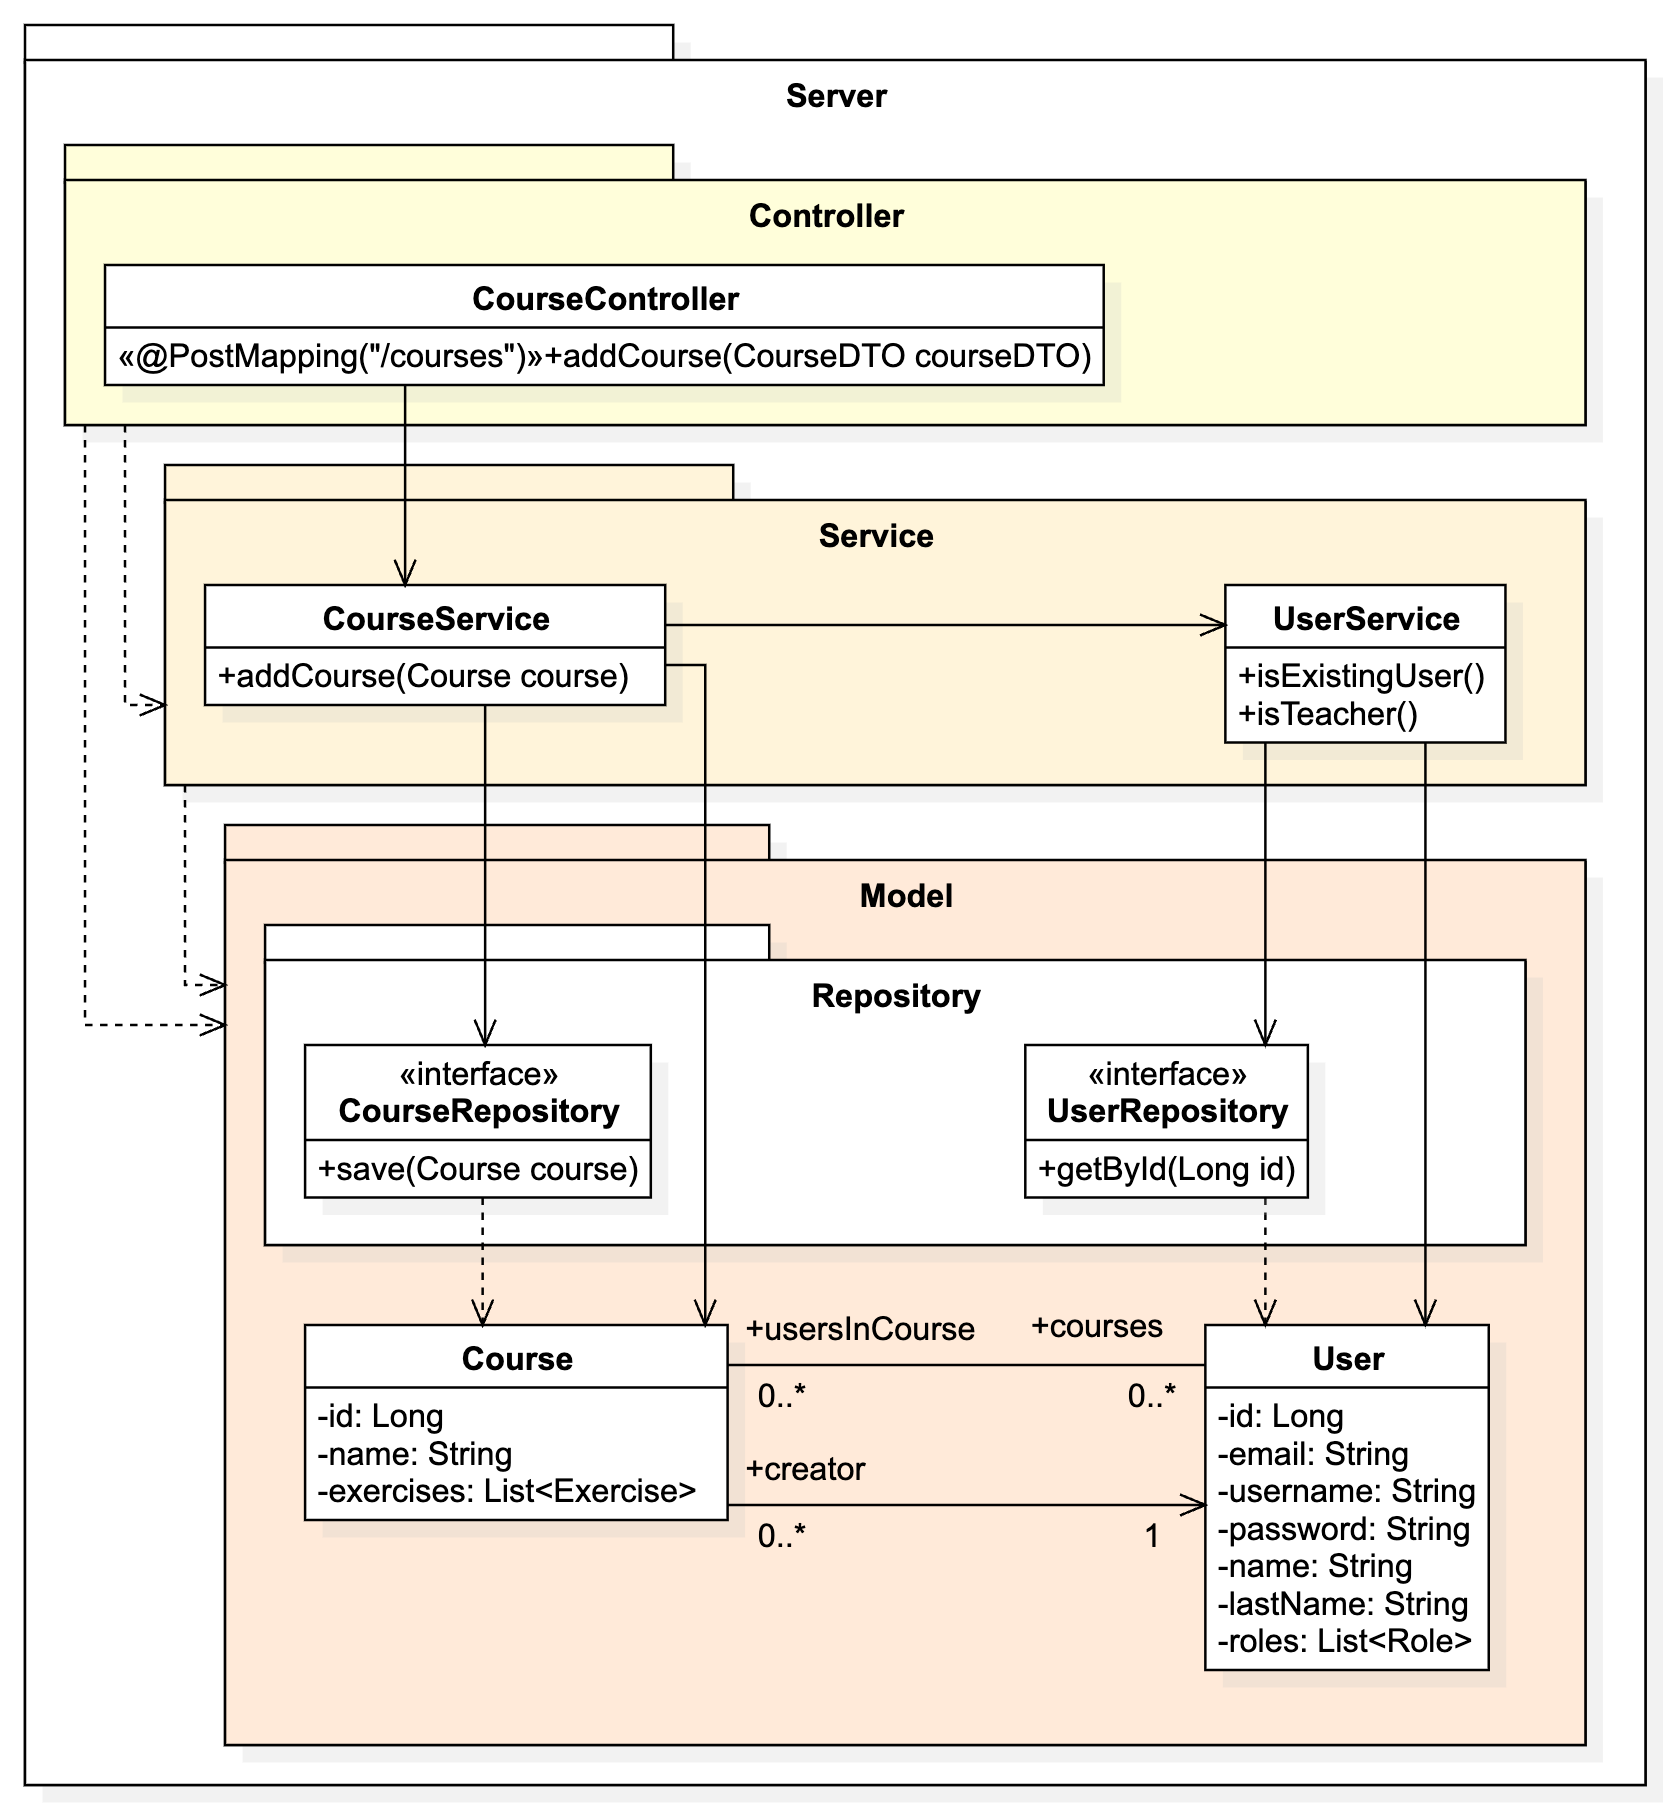
\includegraphics[width=0.8725\textwidth]{imagenes/utilizadas/4-2-arquitectura/diagramas/diag3-mvcServidorEjemplo.png}
    \caption{Diagrama de clases que refleja un fragmento del servidor para ejemplificar el flujo de funcionamiento y las dependencias en MVC.}
    \label{fig:diagMVCServidorEjemplo}
\end{figure}

\subsubsection{Extensión para Visual Studio Code}
\label{subsec:arqCliente}
La extensión para Visual Studio Code es una aplicación basada en la plataforma Node ---tal como se expone en la \referenciaSeccion{subsec:tecCliente}---, y tiene un diseño dividido en cuatro capas principales:
\begin{itemize}
    \item Cliente (paquete \texttt{client}). Contiene todas las clases relativas a la conexión de la extensión con el servidor, relegándose a esta capa la configuración de las peticiones y los parámetros que deben recoger todas ellas como, por ejemplo, el tiempo de expiración o la credencial para la autenticación y autorización del usuario.
    \item Componentes (paquete \texttt{components}). Está conformado por los elementos que se pueden visualizar en la interfaz de usuario del IDE: los ítems de la barra lateral (cursos, ejercicios y otros elementos especiales), el panel web empleado para mostrar el \textit{dashboard} y los botones mostrados en la barra inferior de Visual Studio Code, introduciendo la implementación de sus comportamientos asociados.
    \item Servicios (paquete \texttt{services}). Contiene las implementaciones de algunos servicios, tales como la configuración del sistema de registro de eventos, la capacidad de actualización en tiempo real de la información que el profesor tiene sobre el progreso de los estudiantes o la funcionalidad de registro de comentarios en ficheros.
    \item Modelo (paquete \texttt{model}). De forma análoga al servidor, se introducen en este nivel las clases empleadas por la aplicación para la representación de las entidades del dominio, preservando los nombres y tipos del servidor para permitir la comunicación entre ambos.
\end{itemize}

Además, al tratarse de un proyecto basado en Node y, además, al hacer uso de la API de desarrollo de extensiones de Visual Studio Code \cite{Tec_VSCodeExtAPI}, cabe reseñar la presencia de dos ficheros fundamentales:
\begin{itemize}
    \item \texttt{extension.ts}. Toma el rol de punto de entrada de la extensión y se ocupa de orquestar su funcionamiento. Está fuera de los cuatro niveles desarrollados anteriormente.
    \item \texttt{package.json}. El desarrollo de una extensión para Visual Studio Code exige que, aparte de los datos que habitualmente recoge, se declaren en este fichero los eventos que activan la extensión, la ruta al punto de entrada y las contribuciones de la extensión al IDE, tales como: comandos implementados, opciones de configuración incorporadas y las vistas mostradas al usuario, incluyendo detalles acerca de los tipos de elementos mostrados en la vista lateral, las acciones disponibles o su posición, entre muchas otras cuestiones.
\end{itemize}

\subsubsection{Aplicación web SPA}
\label{subsec:arqAppWeb}
La aplicación web introducida hace uso del \textit{framework} Angular para su funcionamiento ---tal como se desarrolla en la \referenciaSeccion{subsec:tecAppWeb}---. La arquitectura de este componente sigue, al igual que el servidor, una particularización de la arquitectura MVC \cite{Arq_MVCFowler}:
\begin{itemize}
    \item Modelo. Es, al igual que en los otros dos casos, el conjunto de las clases necesarias para la interpretación en términos informáticos del dominio. Están alojadas en la carpeta \texttt{model}.
    \item Controlador. En este caso, está conformado por las clases agrupadas en la carpeta \texttt{services}. En este caso, esta capa incorpora la lógica de negocio mínima requerida para la interpretación de la información intercambiada con el servidor, ocupándose de lanzar peticiones al servidor y de interpretar las respuestas recibidas para, tras adaptarla al modelo de la aplicación, mostrarla mediante los componentes que integran la vista.
    \item Vista. Alojada en la carpeta \texttt{components}, es el conjunto de los componentes, que son la ``unidad básica y principal para la construcción de aplicaciones Angular'' \cite{Arq_AngularComponents}. Están compuestos por tres partes: una plantilla, que determina la estructura del componente para su renderización en un navegador web, una hoja de estilos (opcional) y una clase en TypeScript que define cómo manejar la información que se utilizará en la plantilla, acudiendo a los servicios del controlador para obtenerla o enviarla al servidor.
\end{itemize}

Fuera del código fuente propio de la aplicación, es pertinente destacar algunos ficheros cruciales para el correcto funcionamiento de este componente:
\begin{itemize}
    \item \texttt{index.html}, \texttt{styles.css} y \texttt{main.ts}. Estos tres ficheros, situados en la raíz del componente, son el punto de entrada de la aplicación Angular.
    \item \texttt{package.json}. Es el manifiesto del proyecto, y contiene toda la información relativa al proyecto en tanto que basado en Node: nombre del componente, licencia y dependencias asociadas, así como la versión de Angular empleada y los distintos \textit{scripts} que se pueden ejecutar sobre el proyecto.
    \item \texttt{tsconfig.json}. Es la configuración propia del compilador/transpilador de TypeScript a JavaScript.
    \item \texttt{angular.json}. Es la configuración básica del proyecto Angular.
    \item \texttt{app-routing.module.ts}. Situado dentro del código fuente, este fichero define cómo deben mostrarse los componentes de la vista mediante la instanciación de una clase propia de Angular que permite definir qué componente se debe activar para cada una de las posibles rutas introducidas en la URL \cite{Arq_AngularRouter}.
\end{itemize}
